\documentclass[main]{subfiles}
\begin{document}

%@@@@@@@@@@@@@@@@@@@@@@@@@@@@@@
% Main Topics: set packing, covering, partition, facility location problem
% and spanning trees
% Polyhedral representation of discrete optimization problems - 23.11.2017
% author: Vanessa Leite

\section{Modeling with Discrete Variables}

\subsection{Set covering, packing and partitioning}
\paragraph{Definition: Let $M$ be a finite ground set. $M = \{1, \dots, m\}$.
Given a collection $M_1, \dots, M_n \subseteq M$, $c_j > 0$ is the weight of
subsets $M_j$, $M_j = \{1, \dots, n\}$.}

\subparagraph{Cover:} $J \subseteq \{1, \dots, n\}$ is a cover if $\bigcup_{j
\in J} M_j = M$.

\subparagraph{Packing:} $J \subseteq \{1, \dots, n\}$ is a packing if $M_i \cap
M_j = \emptyset$, $\forall i \in J, i \neq j$.

\subparagraph{Partition:} A partition is a subset $J \subseteq \{1, \dots, n\}$
such that $J$ is a cover and a packing.

\begin{figure}[!h]
  \centering
    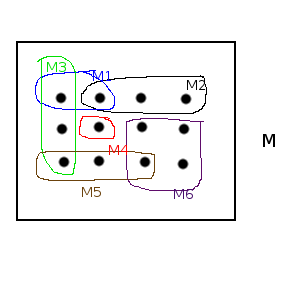
\includegraphics[width=0.3\textwidth]{imgs/partition-set.png}
    \caption{$J = \{2,5\}$ is a packing. There is no partition on this set.}
\end{figure}

\paragraph{The optimization problems:}
\begin{enumerate}
\item Max-weight packing
\item Min-weight cover
\item Min/Max-weight partition
\end{enumerate}

\paragraph{Goal: "translate" these optimization problems into "polyhedral
language".} It requires to find a matrix $A \in \Z^{m \times n}$, where $m$ is
our ground set and $n$ is the subsets of $M$. $A_{ij} = 
\begin{cases}
  0\text{, if } i \notin M_j\\
  1\text{, if } i \in M_j\\
\end{cases}$.

Introduce variables $x_j \forall j \in N$. $x_j \in \{0,1\}$. Each $x_j = 1$
means to select the set.

\begin{enumerate}
\item Max-weight packing: $\max \sum_{j = 1}^n c_j x_j$, $Ax \leq
\mathds{1} \in \R^m$
\item Min-weight cover: $\min \sum_{j = 1}^n c_j x_j$, $Ax \geq
\mathds{1} \in \R^m$
\item Min/Max-weight partition: $\min / \max \sum_{j = 1}^n c_j x_j$, $Ax =
\mathds{1} \in \R^m$, $0 \leq x \leq \mathds{1}$, $x \in \Z^n$
\end{enumerate}


\subsection{Formulations}

\paragraph{Definition - Mixed Integer Optimization Problem (MIP)} Mixed =
integer and continuous variables:
$\max \{\sum c_i x_i + \sum d_j y_j \mid Ax + Dy \leq b, x \in \R^n, y \in
\Z^d\}$.
Its \textbf{linear relaxation} is defined by replacing $y \in \Z^d$ by
$y \in \R^d$.

\paragraph{Example (facility location problem):}
Customers $i \in \{1, \dots, n\}$. Potential facilities $j \in \{1, \dots, m\}
$. We have a fixed cost $c_j$ for opening facility $j$. Variable cost $d_{ij}$
for serving client $i$ from facility $j$ (of course, if it is open).\\
$x_{ij} \in [0,1]$: percentage of serving client $i$ from $j$. For all $i \in
\{1, \dots, n\}$ and $j \in \{1, \dots, m\}$.\\
$y_j \in \{0,1\}$ $\forall j \in \{1, \dots, m\}$ indicates if we open $j$-th
facility.\\
$P_{FL} = \{ \sum_{j =1}^{m} x_{ij} = 1$, $\forall i \in \{1, \dots, n\}$,
$x_{ij} \leq y_j$ $\forall i,j \}$\\
Objective: $Z_{FL} = \min \sum_{j=1}^m c_j y_j + \sum_{i,j} d_{ij} x_{ij}$

We could also look at a second version of the problem:
$P_{AFL} = \{ (x,y) \mid \sum_{j=1}^{m} x_{ij} = 1$, $\forall i$, $\sum_{i=1}^n
x_{ij} \leq n y_j \forall j$, $0 \leq x_{ij} \leq 1$, $0 \leq y_j \leq 1\}$\\
Objective: $Z_{AFL} = \min \sum_{j=1}^m c_j y_j + \sum_{i,j} d_{ij} x_{ij}$,
$(x,y) \in P_{AFL}$.

\emph{Observe: $P_{AFL} \supseteq P_{FL} \supseteq P_{FL} \cap
(\underbrace{\R^{n \times m}}_{x} \times \underbrace{\Z^m}_{y}) = P_{AFL} \cap
(\R^{n \times m} \times \Z^m)$}

$(x,y) \in P_{FL} \rightarrow x_{ij} \leq y_i \forall i \rightarrow
\sum_{i=1}^n x_ij \leq n y_j$

\paragraph{Example (minimum spanning tree):}
Given $G=(V,E)$, weights $w_ij \forall i,j \in E$, $G$ connected, a forest $F
\subseteq E$, $(V,F)$ contains no cycle.

\subparagraph{Definition - spanning tree:} $T \subseteq E$ is a spanning tree
if $(V,T)$ has no cycles and $|T| = n-1$, $n = |V|$.

\subparagraph{Lemma - graph theory:} $T \subseteq E$ is a spanning tree
$\iff |T| = n-1$ and $(V,T)$ is connected.

Two formulations for min-weight spanning trees: variables $x_{ij} \in \{0,1\}
\forall (i,j) \in E$.

\subparagraph{Subtour-elimination formulation (relaxation)}
$P_{SUB} = \{ x \in [0,1]^{|E|} \mid \sum_{e \in E(S)} x_e \leq |S| - 1
\forall S \subseteq V \}$

\emph{Notation: For $S \subseteq V$, $E(S) = \{(i,j) \in E \mid i,j \in S\}$.
$\delta(S) = \{(i,j) \in E \mid i \in S, j \notin S\}$, i.e., a cut comming
from $S$.}

\subparagraph{Optimization problem 1:}
$Z_{SUB} = \min \{ x \in P_{SUB} \cap \Z^n \sum_{e \in E} w_e x_e\}$

\subparagraph{Optimization problem 2 (cut set formulation):}
$P_{cut} = \{ x \in [0,1]^{|E|} \mid \sum_{e \in \delta(S)} x_e \geq 1$,
$\forall \emptyset \neq S \neq V$, $S \subseteq V$.

$Z_{cut} = \min \{ x \in P_{cut} \cap \Z^n \sum_{e \in E} w_e x_e\}$

\paragraph{Theorem:}
\begin{enumerate}
\item $P_{SUB} \subseteq P_{cut}$
\item In general, $P_{SUB} \neq P_{cut}$ and $P_{cut}$ may have non integral
extreme points.
\end{enumerate}

\subparagraph{Proof:}
\begin{enumerate}
\item $x$ in $P_{SUB}$. Show $S \subseteq V$, $S \neq 0$, $S \neq V$,
$\sum_{e \in \delta(S)} x_e \geq 1$.\\
$E = E(S) \cup \delta(S) \cup E(V\S)$. $x \in P_{SUB} \rightarrow \sum_{e \in 
E(S)} x_e \leq |S| - 1$. $\sum_{e \in E(V\S)} x_e \leq |V|-|S|-1 = n-|S|-1$
$\rightarrow n - 1 = \sum_{e \in E(S)} x_e + \sum_{e \in \delta(S)} x_e +
\sum_{e \in E(V\S)} x_e \rightarrow \sum_{e \in \delta(S)} x_e = n-1 -
\underbrace{(\sum_{e \in E(S)} x_e)}_{\leq |S| - 1} - \underbrace{(\sum_{e \in 
E(V\S)} x_e)}_{\leq n-|S|-1} \geq n - 1 - (|S|-1)-(n-|S|-1) = -|S|+|S|+1 =1$
\item 
\end{enumerate}


\end{document}